\chapter{Árvore Binária}
\label{ch:arvore_binaria} % This how you label a chapter and the key (e.g., ch:into) will be used to refer this chapter ``Introduction'' later in the report. 
Para criar uma árvore binária pouco desequilibrada a partir de uma lista de dados de entrada, podemos usar a estratégia de \textbf{divisão e conquista}. A ideia é organizar os dados de entrada, selecionar o elemento do meio como raiz e repetir esse processo para as sub-árvores da esqueda e direita.

\subsection*{Estratégia: Construção Balanceada com Lista Ordenada}

\begin{enumerate}
    \item \textbf{Ordenar os dados de entrada:}
    \begin{itemize}
        \item Se os dados não estiverem ordenados, ordene-os. Isso garante que a árvore seja uma \textit{árvore binária de busca}.
    \end{itemize}

    \item \textbf{Escolher o elemento do meio como raiz:}
    \begin{itemize}
        \item Divida a lista ao meio. O elemento central vai ser a raiz da árvore ou subárvore.
    \end{itemize}

    \item \textbf{Repetir de forma recursiva:}
    \begin{itemize}
        \item Para os elementos à esquerda do meio, crie a subárvore esquerda.
        \item Para os elementos à direita do meio, crie a subárvore direita.
    \end{itemize}

    \item \textbf{Continuar até que a lista esteja vazia:}
    \begin{itemize}
        \item A recursão terminará quando não houverem mais elementos na lista.
    \end{itemize}
\end{enumerate}

\subsection*{Exemplo: Construção da Árvore}
Considere os seguintes dados iniciais:

\[
10, \; 2, \; 5, \; 3, \; 9, \; 7, \; 1, \; 4, \; 6
\]

Primeiro, ordenaremos os valores.

\[
1, \; 2, \; 3, \; 4, \; 5, \; 6, \; 7, \; 9, \; 10
\]

\begin{enumerate}
    \item O nó \textbf{5} é escolhido como raiz da árvore, pois é o elemento central da lista.
    
    \begin{figure}[!ht]
    	\centering
    	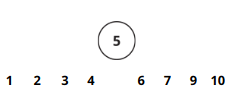
\includegraphics[scale=0.7]{figures/binaria/passo1.png}
    	\label{fig:bubble_sort_example}
    \end{figure}
    
    \item A subárvore esquerda contém os números menores que 5 (\textbf{1, 2, 3, 4}) e a da direita contém os números maiores que 5 (\textbf{6, 7, 9, 10})
    \begin{itemize}
        \item O elemento central (\textbf{2}) é escolhido como a raiz da subárvore esquerda.
        \item O elemento central (\textbf{7}) é escolhido como a raiz da subárvore direita.
    \end{itemize}
    
    \begin{figure}[!ht]
	\centering
	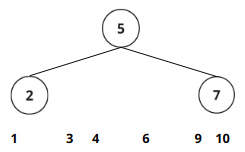
\includegraphics[scale=0.7]{figures/binaria/passo2.png}
	\label{fig:bubble_sort_example}
    \end{figure}
    
    \item Repetimos o processo a partir dos nós 2 e 7
    \begin{itemize}
        \item A subárvore esquerda de 2 contém os números menores que 2 (\textbf{1}) e a da direita contém os números maiores que 2 (\textbf{3, 4})
        \item (\textbf{1}) é escolhido como raíz da árvore esquerda de 2
        \item A subárvore esquerda de 7 contém os números menores que 7 (\textbf{6}) e a da direita contém os números maiores que 7 (\textbf{9, 10})
        \item (\textbf{6}) é escolhido como raíz da árvore esquerda de 7
    \end{itemize}
    
    \begin{figure}[!ht]
	\centering
	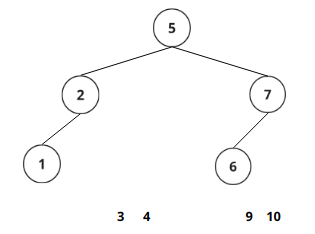
\includegraphics[scale=0.7]{figures/binaria/passo3.png}
	\label{fig:bubble_sort_example}
    \end{figure}
    
    \item Finalizamos a árvore
    \begin{itemize}
        \item O elemento central (\textbf{3}) da árvore direita de 2 é escolhido como a raiz da subárvore direita.
        \item Como (\textbf{4}) é maior que 3, ele será a  raiz da subárvore direita de 3.
        \item O elemento central (\textbf{9}) da árvore direita de 7 é escolhido como a raiz da subárvore direita.
        \item Como (\textbf{10}) é maior que 9, ele será a raiz da subárvore direita de 9.
    \end{itemize}

    \begin{figure}[H]
	\centering
	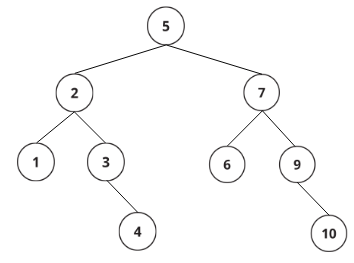
\includegraphics[scale=0.7]{figures/binaria/passo4.png}
	\label{fig:bubble_sort_example}
    \end{figure}
\end{enumerate}
